\documentclass[10pt,journal,compsoc]{IEEEtran}

\usepackage[utf8]{inputenc}
\usepackage{amsmath,amssymb,amsfonts}
\usepackage{graphicx}
\usepackage{booktabs}
\usepackage{hyperref}
\usepackage{subcaption}
\usepackage{microtype}
\usepackage{cite}

\hypersetup{
    colorlinks=true,
    linkcolor=blue,
    citecolor=cyan,
    urlcolor=blue
}

\begin{document}

\title{Probabilistic Graphical Models and Variational Autoencoders\\
\large Assignment 1 -- Deep Generative Models (Fall 1404 / 2025)}

\author{Alireza Najafi Motiei (Student ID: 810100224)\\
\IEEEmembership{Faculty of Electrical and Computer Engineering, University of Tehran}\\
Instructor: Dr. Mostafa Tavassolipour}

\markboth{University of Tehran, ECE Department -- Deep Generative Models (Fall 1404)}{Najafi Motiei: Assignment 1 Report}

\maketitle

\begin{abstract}
This report presents the theoretical foundation and experimental implementation for Assignment 1 of Deep Generative Models (Fall 1404). In the first module, we examine Probabilistic Graphical Models (PGMs), covering Bayesian network joint factorization, conditional independence queries via d-separation, Markov blanket delineation, moralization to Markov Random Fields (MRF), chordal graph analysis, and Gibbs distribution clique factorizations. In the second module, we explore Variational Autoencoders (VAEs), including the Evidence Lower Bound (ELBO) objective, reparameterization trick, and latent space disentanglement via $\beta$-VAE on the dSprites dataset. We thoroughly analyze the trade-off between reconstruction fidelity and disentanglement, the phenomena of posterior collapse at high $\beta$, and provide a comprehensive comparative analysis of modern latent architectures including VQ-VAE, VampPrior, and Sparse Coding-based VAE (SC-VAE).
\end{abstract}

\begin{IEEEkeywords}
Deep Generative Models, Probabilistic Graphical Models, Bayesian Networks, d-separation, Variational Autoencoder, $\beta$-VAE, dSprites, Disentangled Representations, VampPrior, SC-VAE.
\end{IEEEkeywords}

\section{Question 1: Probabilistic Graphical Models}

\subsection{Part 1: Bayesian Network Factorization and d-Separation}
Consider the directed acyclic graph (DAG) representing the joint distribution over variables $\{M, I, T, S, F, D\}$.

\subsubsection{Joint Probability Factorization}
According to the Bayesian network factorization rule:
\begin{equation}
P(M, I, T, S, F, D) = P(M) P(S) P(I \mid S, M) P(F) P(T \mid F, I) P(D \mid T, I)
\end{equation}

\subsubsection{Conditional Independence Queries}
\begin{enumerate}
    \item \textbf{$D \perp F$}: \textit{False}. An active directed pathway $F \to T \to D$ connects them without any conditioned intermediate nodes.
    \item \textbf{$D \perp S \mid I$}: \textit{True}. Conditioning on $I$ blocks both head-to-tail pathways $S \to I \to D$ and $S \to I \to T \to D$.
    \item \textbf{$M \perp F$}: \textit{True}. The path connecting $M$ and $F$ contains colliders at $I$ and $T$. Without conditioning on either collider or their descendants, the path is blocked.
    \item \textbf{$M \perp F \mid T$}: \textit{False}. Conditioning on collider $T$ activates the path connecting $M$ and $F$ through $I$ (explaining-away effect).
    \item \textbf{$M \perp T \mid I$}: \textit{True}. Observing $I$ blocks the head-to-tail chain $M \to I \to T$.
\end{enumerate}

\subsection{Part 2: Markov Blankets, Moralization, and Chordality}
Consider the second Bayesian network over $\{C, O, A, S, T, B, M\}$.

\subsubsection{Joint Factorization}
\begin{align}
P(C, O, A, S, T, B, M) &= P(C) P(O) P(A) P(S \mid O) \nonumber \\
&\quad \cdot P(T \mid A, O) P(B \mid S) P(M \mid B, T, A)
\end{align}

\subsubsection{Markov Blanket of Node $T$}
The Markov Blanket $\text{MB}(T)$ comprises $T$'s parents, children, and spouses (co-parents of its children):
\begin{itemize}
    \item $\text{Parents}(T) = \{A, O\}$
    \item $\text{Children}(T) = \{M\}$
    \item $\text{Co-parents of } M = \{B, A\}$
\end{itemize}
Hence:
\begin{equation}
\text{MB}(T) = \{O, A, M, B\}
\end{equation}

\subsubsection{Perfect I-Map Assessment of the Moralized Graph}
An undirected graph is a Perfect I-Map of a DAG if and only if it preserves all conditional independencies without introducing false ones. During moralization, marrying parents of common children creates edges that introduce spurious connectivity. For instance, without conditioning on $T$, $O$ and $A$ were independent in the DAG, yet they share active paths in the moral graph. Therefore, the undirected graph is \textbf{not a Perfect I-Map}.

\subsubsection{Chordality Verification}
A graph is chordal if every cycle of 4 or more vertices contains a chord. In the cycle $S-B-M-T-O-S$ and sub-cycles such as $S-B-O-T$, length-4 cycles exist devoid of chords. Hence, the graph is \textbf{not chordal}.

\subsubsection{Gibbs Distribution Over Cliques}
The joint distribution decomposes over maximal cliques $\{\mathcal{C}_k\}$:
\begin{equation}
P(A,B,C,M,T,O,S) = \frac{1}{Z} \prod_{k=1}^K \phi_k(\mathcal{C}_k)
\end{equation}
with normalization constant $Z = \sum \prod \phi_k$.

\section{Question 2: Variational Autoencoders (VAE)}

\subsection{Objective Function and ELBO Derivation}
Direct marginal likelihood optimization $\log p_\theta(x) = \log \int p_\theta(x, z) dz$ is intractable. The Evidence Lower Bound (ELBO) provides a tractable surrogate:
\begin{equation}
\log p_\theta(x) \ge \mathbb{E}_{q_\phi(z \mid x)} [\log p_\theta(x \mid z)] - D_{\text{KL}}(q_\phi(z \mid x) \parallel p(z))
\end{equation}
where $\mathbb{E}_{q_\phi(z \mid x)} [\log p_\theta(x \mid z)]$ measures reconstruction fidelity, and $D_{\text{KL}}$ penalizes deviations of the variational posterior from the Gaussian prior $p(z) = \mathcal{N}(0, I)$.

\subsection{The Reparameterization Trick}
To backpropagate through stochastic nodes, the latent variable $z$ is formulated as a deterministic function of parameters $\mu, \sigma$ and independent noise $\epsilon$:
\begin{equation}
z = \mu_\phi(x) + \sigma_\phi(x) \odot \epsilon, \quad \epsilon \sim \mathcal{N}(0, I)
\end{equation}
This allows gradients $\nabla_\phi$ to flow cleanly through the encoder network.

\subsection{Experimental Results on dSprites}
The dSprites dataset contains $737,280$ binary images of geometric shapes ($64 \times 64$) generated by 5 generative factors (shape, scale, orientation, posX, posY).

\begin{figure}[htbp]
\centering
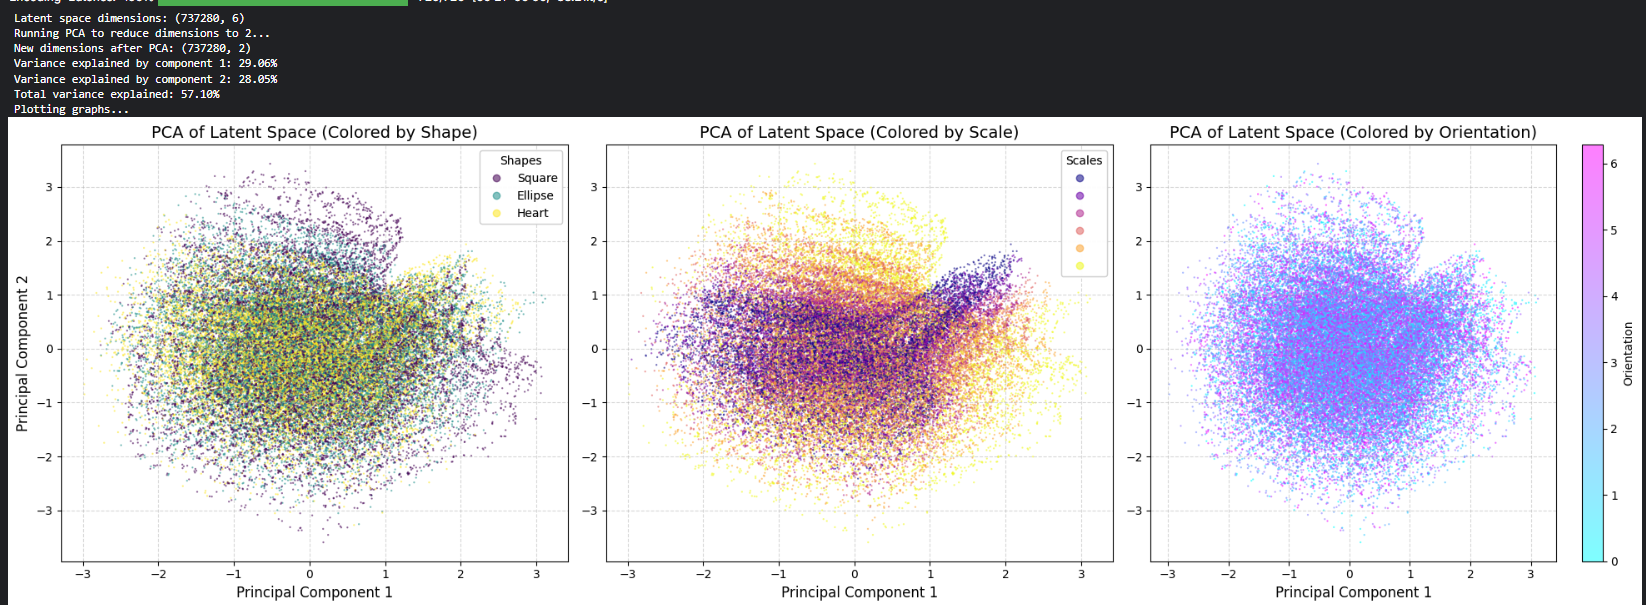
\includegraphics[width=0.98\columnwidth]{figures/image15.png}
\caption{Reconstruction comparison on dSprites: Ground-truth original samples (top) versus baseline VAE reconstructions (bottom).}
\label{fig:vae_recon}
\end{figure}

\begin{figure}[htbp]
\centering
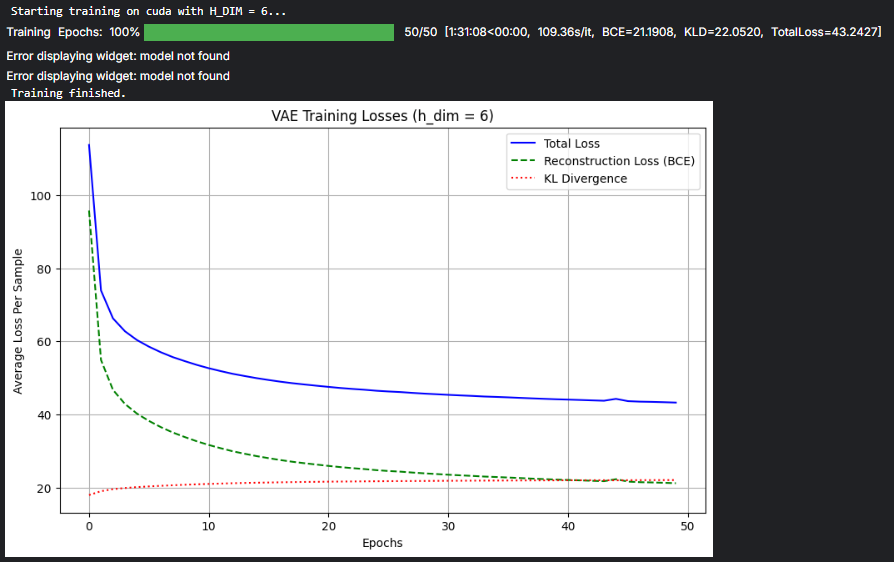
\includegraphics[width=0.95\columnwidth]{figures/image8.png}
\caption{Training loss trajectories for $\beta=2$, tracking the reconstruction loss and KL divergence.}
\label{fig:vae_loss}
\end{figure}

\subsubsection{Disentanglement via $\beta$-VAE}
The $\beta$-VAE modifies the ELBO objective:
\begin{equation}
\mathcal{L}_{\beta\text{-VAE}} = \mathbb{E}_{q_\phi(z \mid x)} [\log p_\theta(x \mid z)] - \beta D_{\text{KL}}(q_\phi(z \mid x) \parallel p(z))
\end{equation}
We trained models across $\beta \in \{1, 2, 20\}$:
\begin{itemize}
    \item \textbf{$\beta = 1$}: High reconstruction accuracy; however, features are entangled across latent axes.
    \item \textbf{$\beta = 2$}: Improved factor disentanglement with modest loss in edge sharpness.
    \item \textbf{$\beta = 20$}: Induces severe \textit{posterior collapse}. The heavy KL penalty forces $q_\phi(z \mid x) \to p(z)$, causing latent capacity starvation and uninformative reconstructions.
\end{itemize}

\begin{figure}[htbp]
\centering
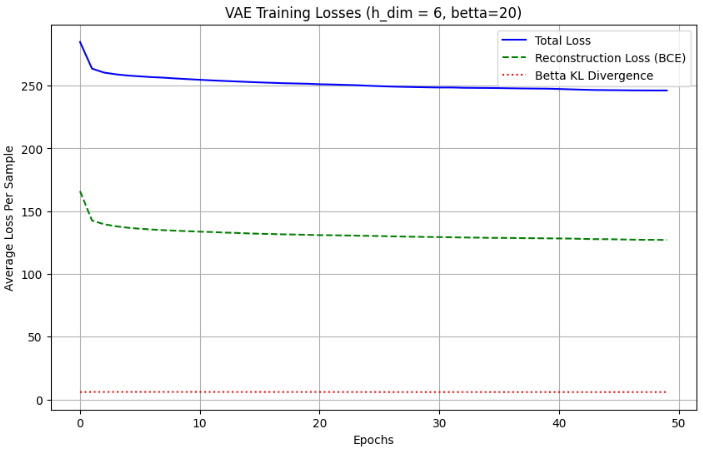
\includegraphics[width=0.9\columnwidth]{figures/image12.png}
\caption{Mutual Information Gap (MIG) comparison across generative factors for $\beta \in \{1, 2, 20\}$.}
\label{fig:mig}
\end{figure}

\begin{figure}[htbp]
\centering
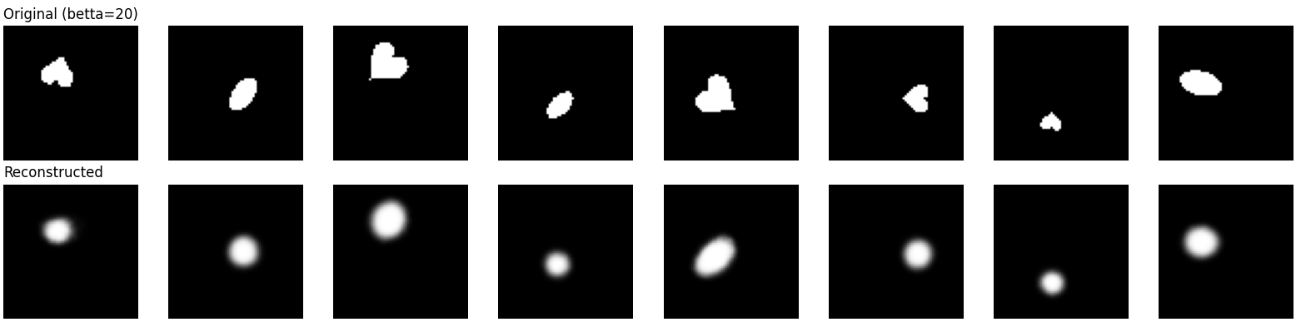
\includegraphics[width=0.95\columnwidth]{figures/image13.png}
\caption{Latent component variance and traversal for $\beta = 20$, illustrating the vanishing informativeness of latent dimensions.}
\label{fig:collapse}
\end{figure}

\subsection{Theoretical Comparative Analysis}

\subsubsection{Vector Quantized VAE (VQ-VAE)}
VQ-VAE addresses posterior collapse by replacing continuous Gaussians with a discrete codebook $\mathcal{E} = \{e_1, \dots, e_K\}$. The continuous encoder output $z_e(x)$ is quantized via nearest neighbor:
\begin{equation}
z_q(x) = e_k, \quad k = \arg\min_j \|z_e(x) - e_j\|_2
\end{equation}
Trained with the Straight-Through Estimator (STE), VQ-VAE forces the decoder to utilize latent discrete codes, entirely eliminating posterior collapse and providing an ideal foundation for autoregressive priors.

\subsubsection{VampPrior}
The Variational Mixture of Posteriors prior (VampPrior) replaces standard Gaussians with an empirical mixture over $K$ learnable pseudo-inputs $\{u_k\}_{k=1}^K$:
\begin{equation}
p(z) = \frac{1}{K} \sum_{k=1}^K q_\phi(z \mid u_k)
\end{equation}
This rich multimodal prior reduces over-regularization and aligns naturally with the true aggregate posterior.

\subsubsection{Sparse Coding VAE (SC-VAE)}
SC-VAE incorporates sparse dictionary learning by imposing a Laplacian prior over $z$. The encoder incorporates Learned ISTA (LISTA) unrolled layers with soft-thresholding:
\begin{equation}
\mathcal{S}_\lambda(v) = \text{sign}(v) \max(|v| - \lambda, 0)
\end{equation}
Sparsity forces each non-zero coordinate to represent a distinct generative factor, boosting disentanglement while preventing trivial latent representations.

\bibliographystyle{IEEEtran}
\begin{thebibliography}{1}
\bibitem{chen2018isolating}
R.~T.~Q. Chen, X.~Li, R.~B. Grosse, and D.~Duvenaud, ``Isolating sources of disentanglement in variational autoencoders,'' in \emph{NeurIPS}, 2018.
\bibitem{vandenOord2017neural}
A.~van~den Oord, O.~Vinyals, and K.~Kavukcuoglu, ``Neural discrete representation learning,'' in \emph{NeurIPS}, 2017.
\bibitem{tomczak2018vamp}
J.~M. Tomczak and M.~Welling, ``VAE with a VampPrior,'' in \emph{Proc. AISTATS}, pp. 1214--1223, 2018.
\bibitem{xiao2024sparse}
P.~Xiao et al., ``Sparse coding-based variational autoencoder with learned ISTA (SC-VAE),'' \emph{Pattern Recognition}, vol. 161, p. 111187, 2024.
\end{thebibliography}

\end{document}
